\subsection{Configuração do Cliente Outlook 2007}

Para configurar a conta de email no Outlook 2007\footnote{A configuração de versões anteriores do Outlook (2000, XP e 2003) é análoga.} deverá ir ao menu tools e seguidamente escolher a opção ``Account Settings'' tal como na seguinte imagem.

\begin{figure}[H]
    \begin{center}
        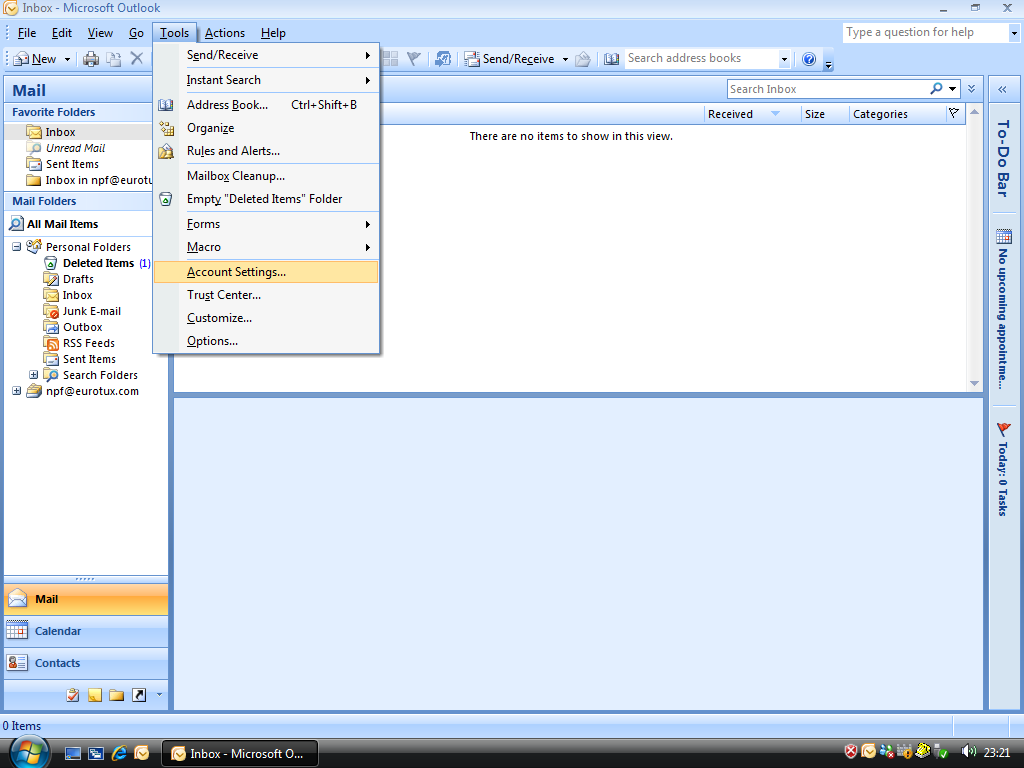
\includegraphics[width=10cm]{include/img/outlook2007_1}
    \end{center}
    \caption{Ecrã inicial Outlook 2007}
    \label{fig:OUTLK2k71}
\end{figure}

De seguida deverá escolher na secção "E-mail" o botão "New" como a imagem seguinte:

\begin{figure}[H]
    \begin{center}
        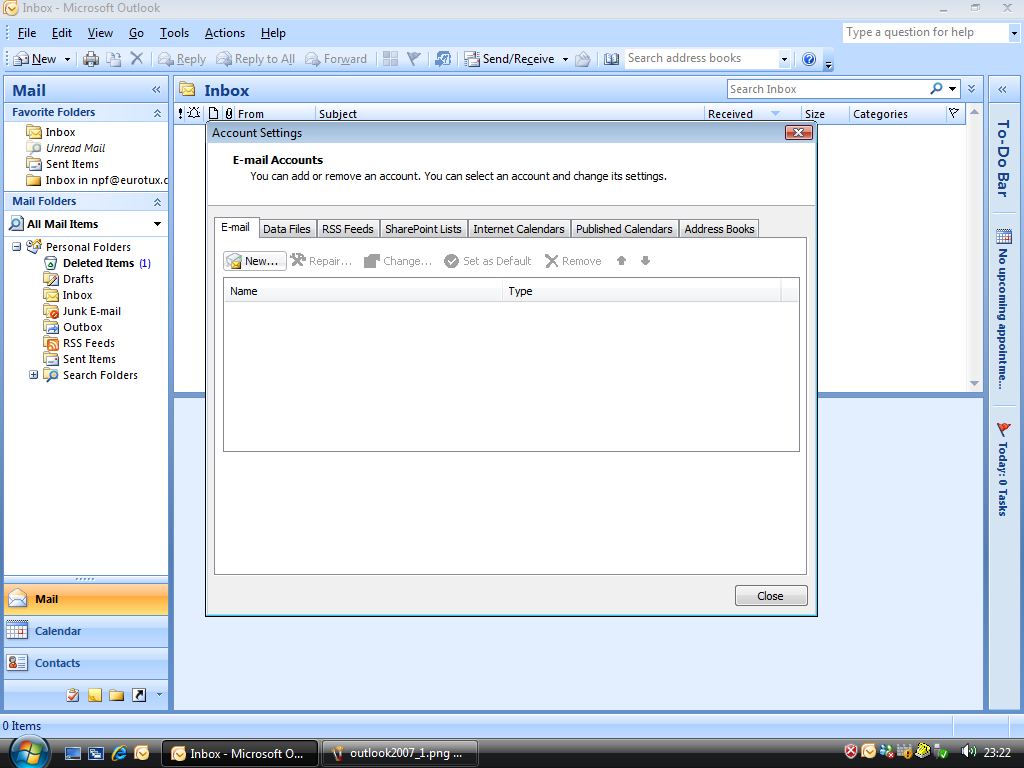
\includegraphics[width=10cm]{include/img/outlook2007_2}
    \end{center}
    \caption{Criação de conta de email - 1}
    \label{fig:OUTLK2k72}
\end{figure}

Na caixa "Add New E-Mail Account" deve escolher em baixo a opção "Manualy configure server settings or aditional server types" e carregar no botão "Next".

\begin{figure}[H]
    \begin{center}
        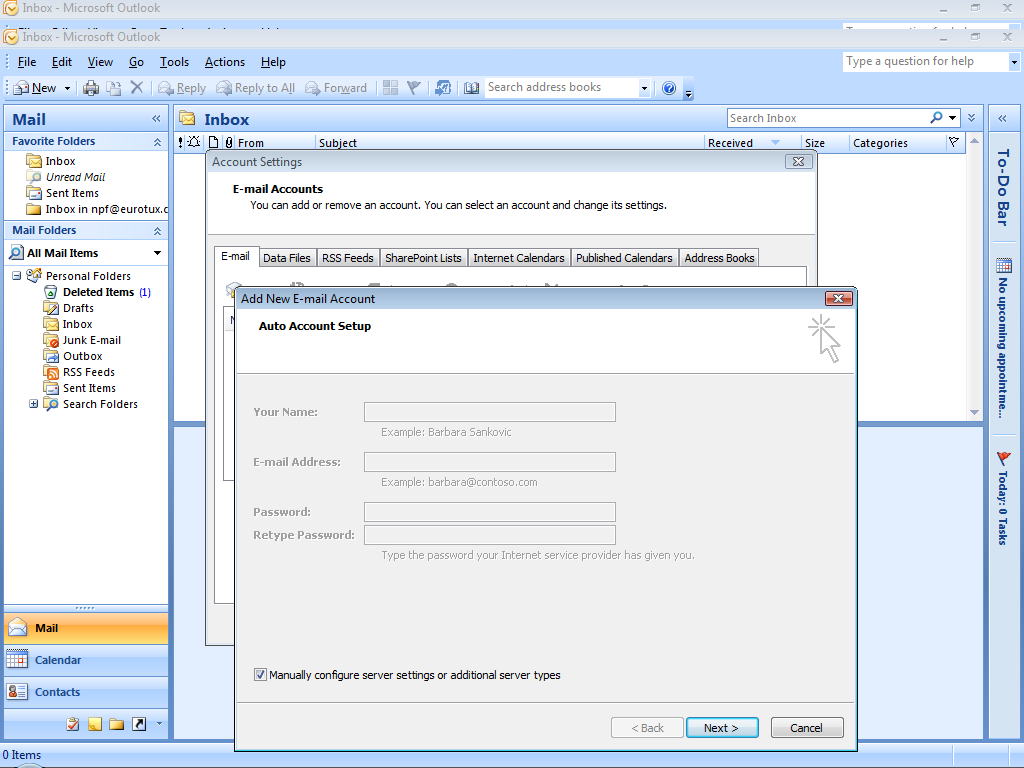
\includegraphics[width=10cm]{include/img/outlook2007_3}
    \end{center}
    \caption{Criação de conta de email - 2}
    \label{fig:OUTLK2k733}
\end{figure}

Escolher a opção "Internet E-Mail" e carregar em "Next".

\begin{figure}[H]
    \begin{center}
        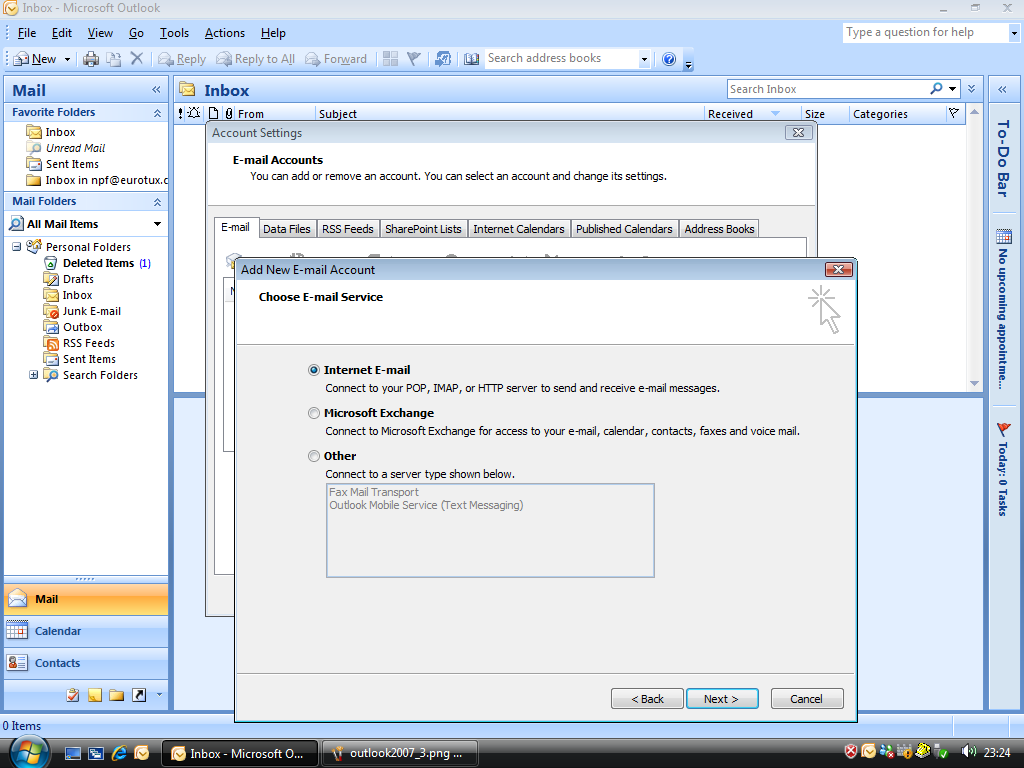
\includegraphics[width=10cm]{include/img/outlook2007_4}
    \end{center}
    \caption{Criação de conta de email - 3}
    \label{fig:OUTLK2k74}
\end{figure}

Inserir na caixa "User Name" o seu nome, na caixa "E-mail Address" o endereço de email que será algo como utilizador@dominio.pt. Poderá variar consoante o seu endereço de correio.

Na combo-box "Account Type" deverá escolher POP3 ou IMAP, na caixa "Incoming mail server" deverá inserir o endereço do seu servidor de email, algo como "mail.dominio.pt". Este endereço poderá variar.

Na caixa "Outgoing mail server" deverá inserir o servidor de correio para enviar. Caso não seja indicado nada em contrário deverá inserir o mesmo que escreveu no "Incoming mail server".

Na caixa "User Name" deverá inserir o seu endereço de email novamente enquanto que na caixa "Password" deverá inserir a sua palavra-passe. Poderá escolher a opção "Remember password". De seguida deverá carregar no botão "More settings".

\begin{figure}[H]
    \begin{center}
        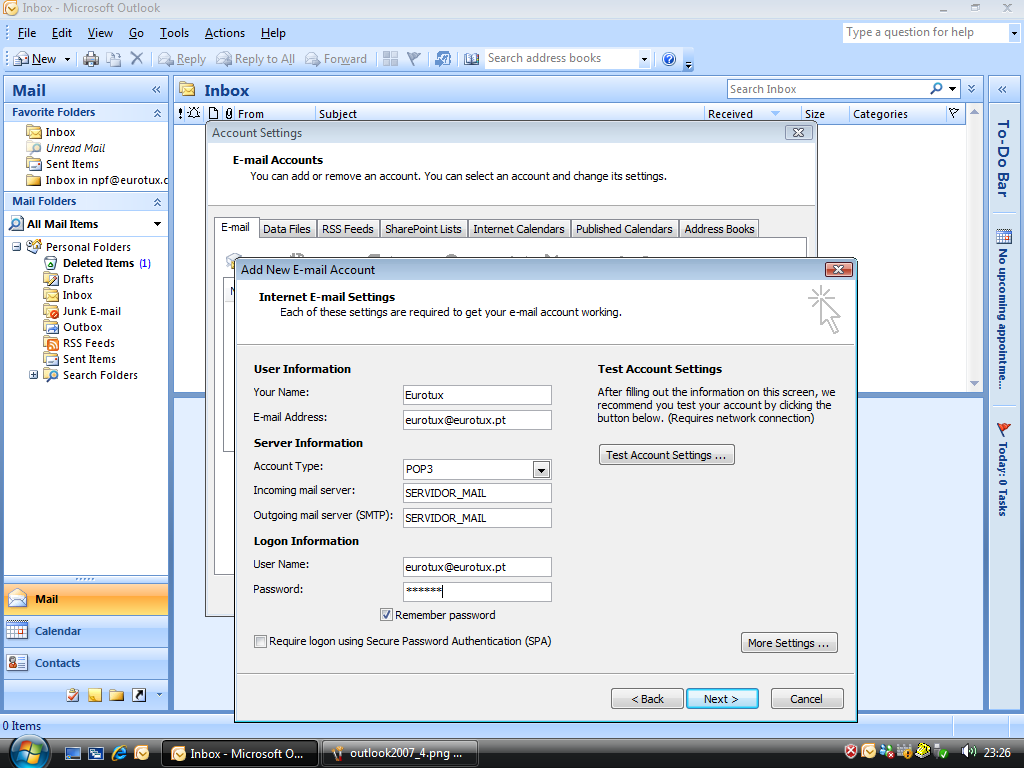
\includegraphics[width=10cm]{include/img/outlook2007_5}
    \end{center}
    \caption{Criação de conta de email - 4}
    \label{fig:OUTLK2k75}
\end{figure}

Na caixa "Internet E-mail Settings" deverá escolher a secção "Outgoing server" e escolher a opção "My outgoing server (SMTP) requires autentication" e a opção "Use same settings as my incoming mail server". De seguida deverá entrar na secção "Advanced".

\begin{figure}[H]
    \begin{center}
        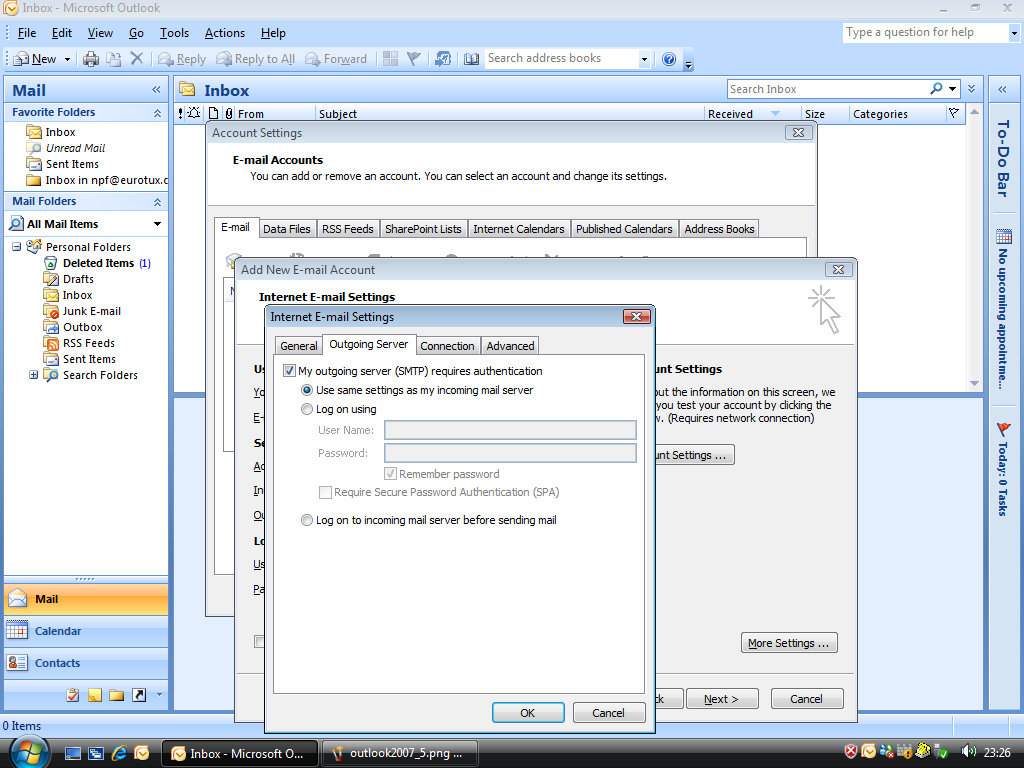
\includegraphics[width=10cm]{include/img/outlook2007_6}
    \end{center}
    \caption{Criação de conta de email - 5}
    \label{fig:OUTLK2k76}
\end{figure}

Na secção "Advanced" no incoming server deverá escolher a opção "This server requires and encrypted connection (SSL)". Note que a porta automaticamente irá mudar para 995 (no caso de ter escolhido anteriormente o POP3) ou 993 (no caso de ter escolhido anteriormente IMAP). Deverá de seguida carregar no botão "OK".

\begin{figure}[H]
    \begin{center}
        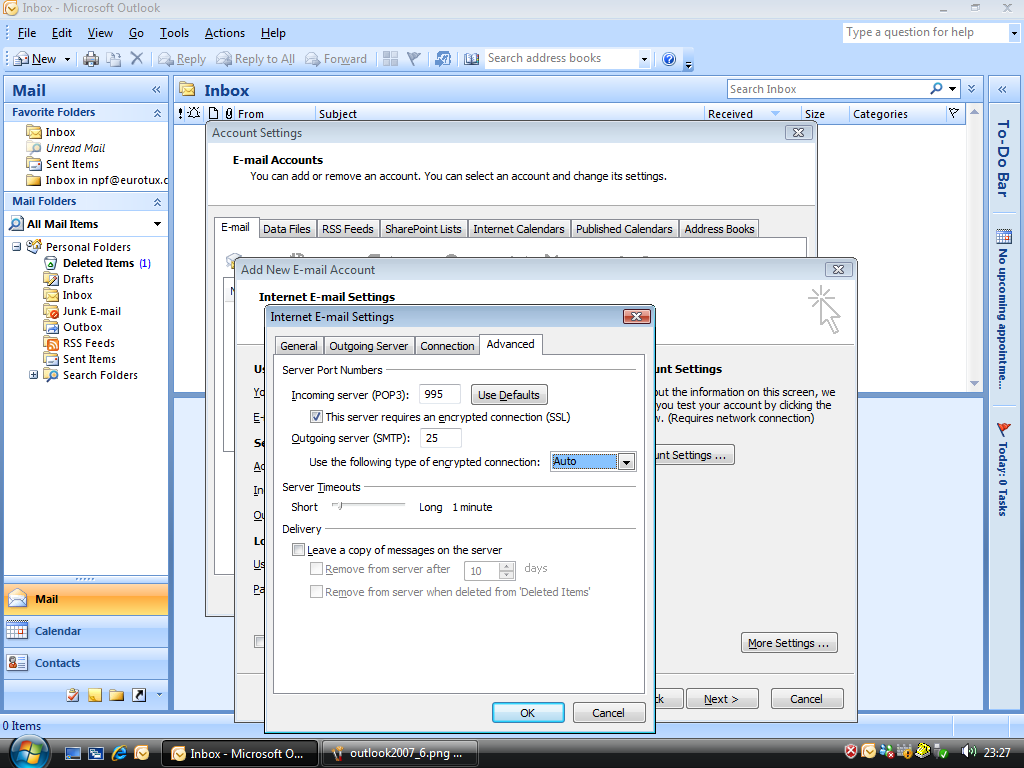
\includegraphics[width=10cm]{include/img/outlook2007_7}
    \end{center}
    \caption{Criação de conta de email - 6}
    \label{fig:OUTLK2k77}
\end{figure}

Deverá carregar agora no botão "Finish" para terminar a criação da conta de correio.

\begin{figure}[H]
    \begin{center}
        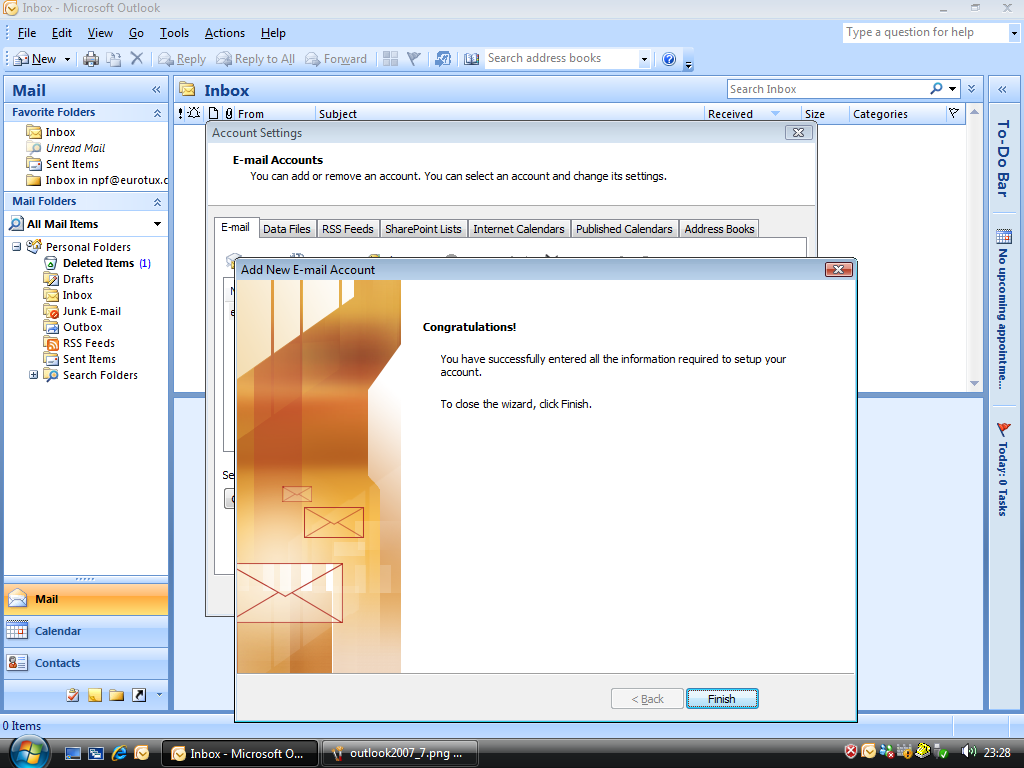
\includegraphics[width=10cm]{include/img/outlook2007_8}
    \end{center}
    \caption{Criação de conta de email - 7}
    \label{fig:OUTLK2k78}
\end{figure}

Ser-lhe-á apresentado um ecrã similar ao seguinte com a conta de correio criada. Deverá carregar em "Close" para fechar a gestão das contas de correio.

\begin{figure}[H]
    \begin{center}
        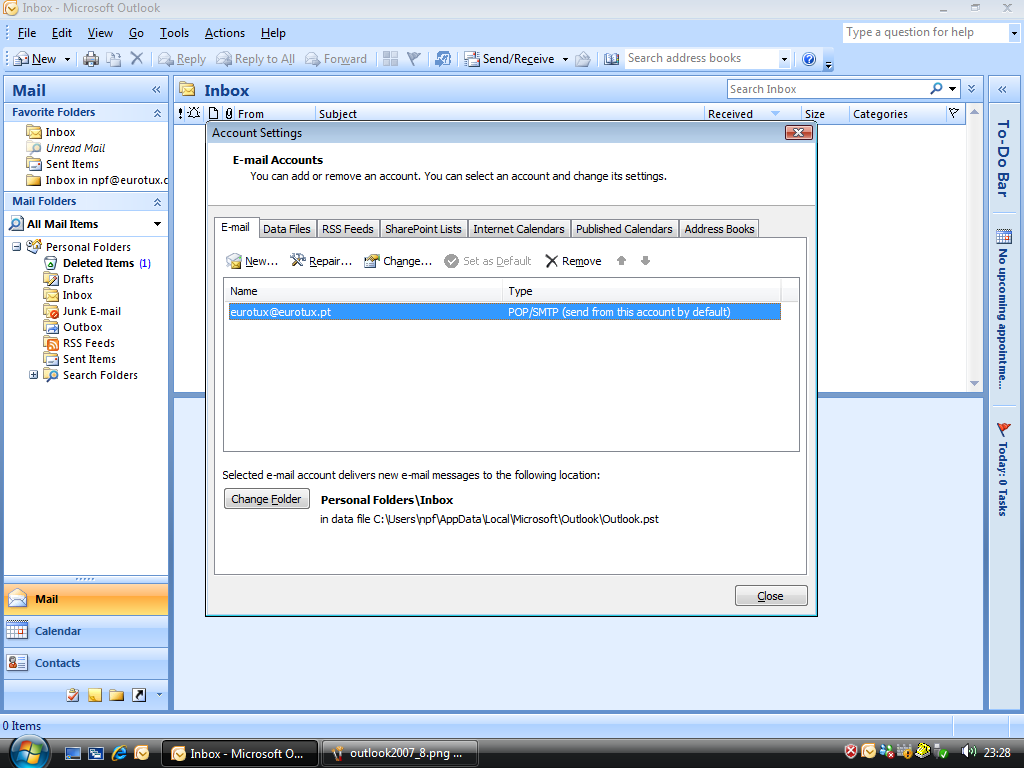
\includegraphics[width=10cm]{include/img/outlook2007_9}
    \end{center}
    \caption{Criação de conta de email - 8}
    \label{fig:OUTLK2k79}
\end{figure}

Quando estiver a escrever um email deverá ter em atenção (no caso de ter várias contas de correio configuradas no mesmo outlook) para enviar pela conta de correio correcta.

\begin{figure}[H]
    \begin{center}
        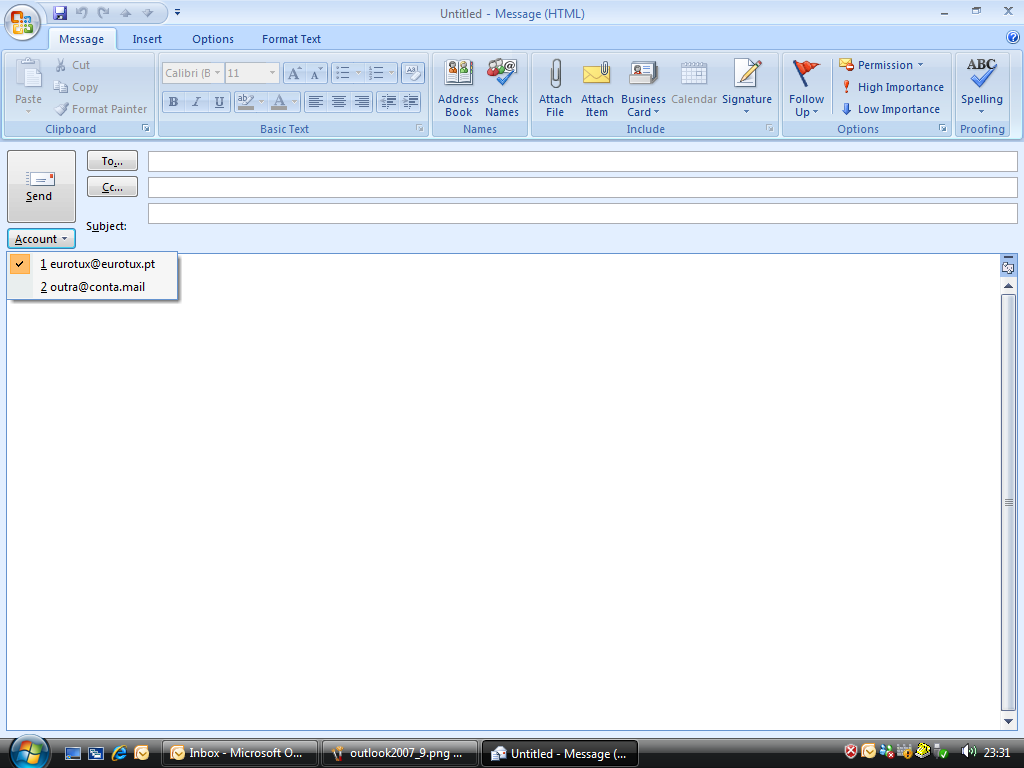
\includegraphics[width=10cm]{include/img/outlook2007_10}
    \end{center}
    \caption{Envio de email}
    \label{fig:OUTLK2k710}
\end{figure}

